The four-GPU pressure sweep varies request rate and average prompt length for
three worker assignments: decode-heavy \texttt{P1/D3}, balanced \texttt{P2/D2},
and prefill-heavy \texttt{P3/D1}. Figure~\ref{fig:pressure} shows the 12 rps
slice. At short prompts, \texttt{P1/D3} has the lowest TTFT.
At the longest prompt point, \texttt{P2/D2} is best because
input pressure dominates. The slowest long-prompt point is \texttt{P1/D3},
reaching 376.5 ms TTFT.

\begin{figure}[t]
\centering
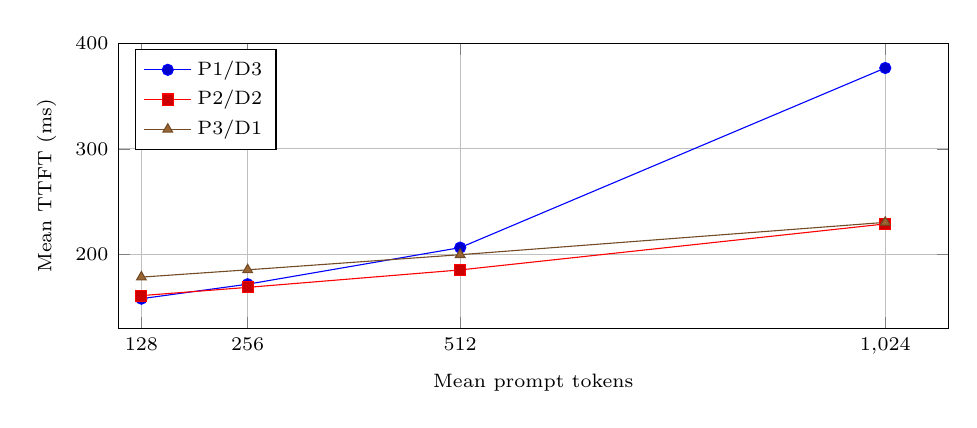
\begin{tikzpicture}
\begin{axis}[
    width=\columnwidth,
    height=2.05in,
    xlabel={Mean prompt tokens},
    ylabel={Mean TTFT (ms)},
    xmin=100,
    xmax=1100,
    ymin=130,
    ymax=400,
    xtick={128,256,512,1024},
    legend style={at={(0.02,0.98)},anchor=north west,font=\scriptsize},
    tick label style={font=\scriptsize},
    label style={font=\scriptsize},
    grid=major
]
	\addplot+[mark=*] coordinates {(128,158.3) (256,172.0) (512,206.6) (1024,376.5)};
\addplot+[mark=square*] coordinates {(128,161.2) (256,169.0) (512,185.5) (1024,229.0)};
\addplot+[mark=triangle*] coordinates {(128,178.7) (256,185.6) (512,199.9) (1024,230.5)};
	\legend{P1/D3,P2/D2,P3/D1}
\end{axis}
\end{tikzpicture}
\caption{Four-GPU pressure sweep at 12 rps. Balanced and prefill-heavy
	assignments trade places as prompt pressure changes. All plotted points are
	extrapolated.}
\label{fig:pressure}
\end{figure}

\begin{figure}[t]
\centering
\resizebox{\columnwidth}{!}{%
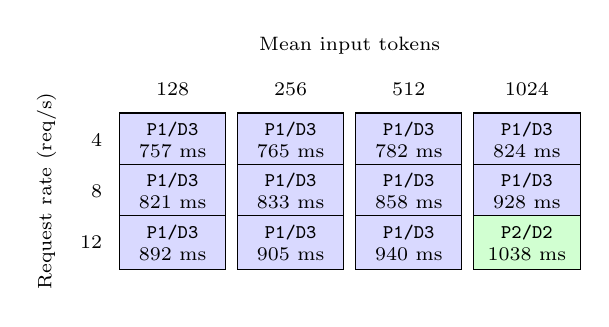
\begin{tikzpicture}[font=\scriptsize]
\node at (3.80,0.55) {Mean input tokens};
\node[rotate=90] at (-0.05,-1.30) {Request rate (req/s)};
\node at (1.55,0) {128};
\node at (3.05,0) {256};
\node at (4.55,0) {512};
\node at (6.05,0) {1024};
\node[anchor=east] at (0.78,-0.65) {4};
\node[anchor=east] at (0.78,-1.30) {8};
\node[anchor=east] at (0.78,-1.95) {12};
\node[draw,fill=blue!15,minimum width=1.35cm,minimum height=0.55cm,align=center] at (1.55,-0.65) {\texttt{P1/D3}\\757 ms};
\node[draw,fill=blue!15,minimum width=1.35cm,minimum height=0.55cm,align=center] at (3.05,-0.65) {\texttt{P1/D3}\\765 ms};
\node[draw,fill=blue!15,minimum width=1.35cm,minimum height=0.55cm,align=center] at (4.55,-0.65) {\texttt{P1/D3}\\782 ms};
\node[draw,fill=blue!15,minimum width=1.35cm,minimum height=0.55cm,align=center] at (6.05,-0.65) {\texttt{P1/D3}\\824 ms};
\node[draw,fill=blue!15,minimum width=1.35cm,minimum height=0.55cm,align=center] at (1.55,-1.30) {\texttt{P1/D3}\\821 ms};
\node[draw,fill=blue!15,minimum width=1.35cm,minimum height=0.55cm,align=center] at (3.05,-1.30) {\texttt{P1/D3}\\833 ms};
\node[draw,fill=blue!15,minimum width=1.35cm,minimum height=0.55cm,align=center] at (4.55,-1.30) {\texttt{P1/D3}\\858 ms};
\node[draw,fill=blue!15,minimum width=1.35cm,minimum height=0.55cm,align=center] at (6.05,-1.30) {\texttt{P1/D3}\\928 ms};
\node[draw,fill=blue!15,minimum width=1.35cm,minimum height=0.55cm,align=center] at (1.55,-1.95) {\texttt{P1/D3}\\892 ms};
\node[draw,fill=blue!15,minimum width=1.35cm,minimum height=0.55cm,align=center] at (3.05,-1.95) {\texttt{P1/D3}\\905 ms};
\node[draw,fill=blue!15,minimum width=1.35cm,minimum height=0.55cm,align=center] at (4.55,-1.95) {\texttt{P1/D3}\\940 ms};
\node[draw,fill=green!18,minimum width=1.35cm,minimum height=0.55cm,align=center] at (6.05,-1.95) {\texttt{P2/D2}\\1038 ms};
\end{tikzpicture}%
}
\caption{Lowest-E2E prefill/decode assignment for a four-GPU server across
request rate and mean input-prompt length. Each cell shows the winning split and mean
E2E latency. All cells are extrapolated.}
\label{fig:pressure-matrix}
\end{figure}

Figure~\ref{fig:pressure-matrix} summarizes the
workload-pressure result. In the request-rate/input matrix, \texttt{P2/D2}
wins 1 cell, \texttt{P3/D1} wins
0 cells, and \texttt{P1/D3} wins
11 cells. This is the stage-balance model in
practice: prompt-heavy regimes prefer prefill capacity, while balanced load
keeps the split near \texttt{P2/D2}. The fixed-rate input/output crossover
matrix is reported with the lowest-E2E global winner rule in
Appendix~\ref{app:global-crossover-matrix}.
